\chapter{Results}
show all views results.
differece of this shader compared to evaluation shader
show real snake images for comparison with real rendered images
show experiments received
show rendered images by daljits implemetation of stams approach.
show our renderer's results 
mention all input parameters and their values.
mention system specs and how long it took in order to precompute
show some idft2 images, used patch, besids rendered image
what initial size was used patch?
mention GEM results.
mention real results from geneva - use same paramter setup.


\section{BRDF maps}
ADD ALOT OF TEXT

% brdf maps patches
\begin{figure}[ht]
  \centering
  \subfigure[Blaze grating]{
    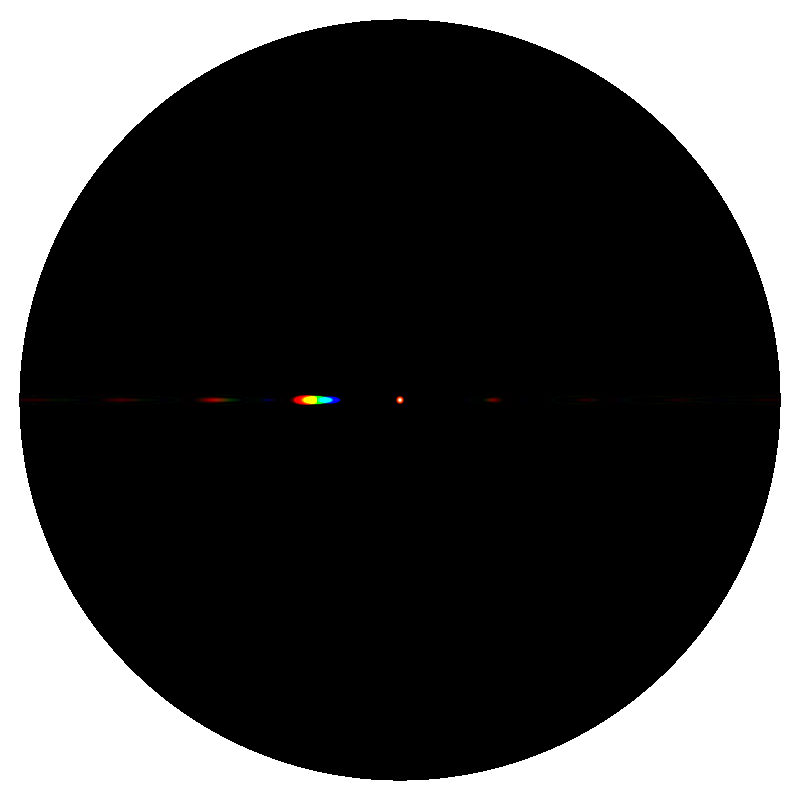
\includegraphics[scale=0.12]{results/diffPatches/fftBlazeHeight_0.25Microns_allL_weak_scale.png}
    \label{fig:brdfmapBlaze}
  }
~
  \subfigure[elaphe grating]{
    \includegraphics[scale=0.12]{results/diffPatches/elaph65.png}
    \label{fig:brdfmapElaphe}
  }
~
  \subfigure[xeno grating]{
    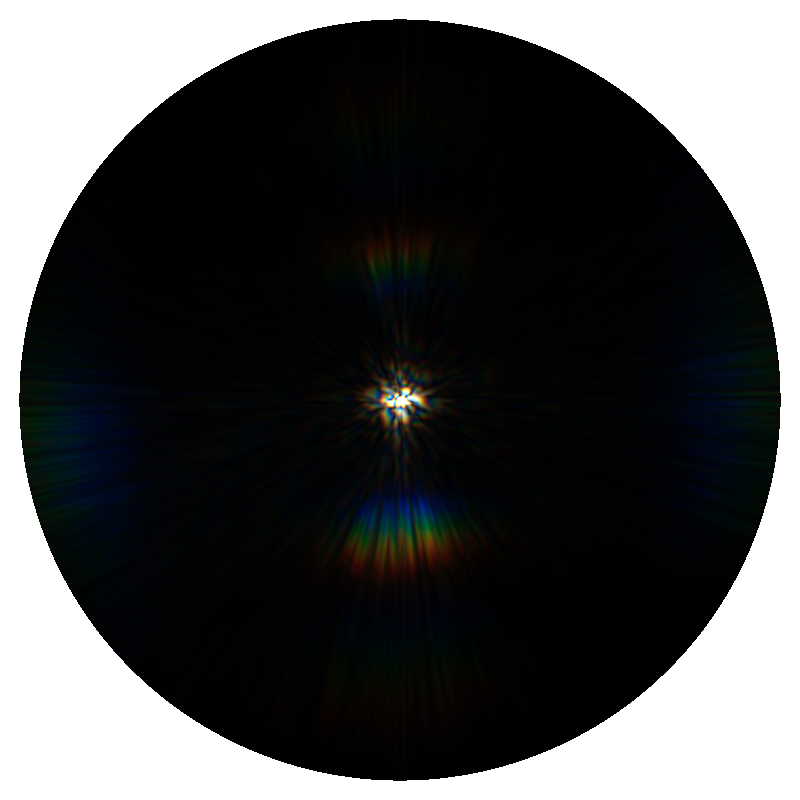
\includegraphics[scale=0.12]{results/diffPatches/xeno65.png}
    \label{fig:brdfmapXeno}
  }
  \label{brdfmapsDiffPatches}
  \caption{BRDF maps for different patches}
\end{figure}


% blaze steps
\begin{figure}[ht]
  \centering
  \subfigure[$\lambda_{step=1 nm}$]{
    \includegraphics[scale=0.12]{results/different_lambda_steps/blaze/dl=1.png}
    \label{fig:brdfmapsDiffLambdaStepsL1Blaze}
  }
~
  \subfigure[$\lambda_{step=5 nm}$]{
    \includegraphics[scale=0.12]{results/different_lambda_steps/blaze/dl=5.png}
    \label{fig:brdfmapsDiffLambdaStepsL5Blaze}
  }
~
  \subfigure[$\lambda_{step=10 nm}$]{
    \includegraphics[scale=0.12]{results/different_lambda_steps/blaze/dl=10.png}
    \label{fig:brdfmapsDiffLambdaStepsL10Blaze}
  }
  
  \subfigure[$\lambda_{step=25 nm}$]{
    \includegraphics[scale=0.12]{results/different_lambda_steps/blaze/dl=25.png}
    \label{fig:brdfmapsDiffLambdaStepsL25Blaze}
  }
~
  \subfigure[$\lambda_{step=50 nm}$]{
    \includegraphics[scale=0.12]{results/different_lambda_steps/blaze/dl=50.png}
    \label{fig:brdfmapsDiffLambdaStepsL50Blaze}
  }
~ 
  \subfigure[$\lambda_{step=100 nm}$]{
    \includegraphics[scale=0.12]{results/different_lambda_steps/blaze/dl=100.png}
    \label{fig:brdfmapsDiffLambdaStepsL100Blaze}
  }
  
  \label{brdfmapsDiffLambdaStepsBlaze}
  \caption{Blaze grating at $2.5 \mu m$: Different $\lambda$ step sizes}
\end{figure}

% elpahe steps
\begin{figure}[ht]
  \centering
  \subfigure[$\lambda_{step=1 nm}$]{
    \includegraphics[scale=0.12]{results/different_lambda_steps/elaphe65/dl=1.png}
    \label{fig:brdfmapsDiffLambdaStepsL1Elaphe65}
  }
~
  \subfigure[$\lambda_{step=5 nm}$]{
    \includegraphics[scale=0.12]{results/different_lambda_steps/elaphe65/dl=5.png}
    \label{fig:brdfmapsDiffLambdaStepsL5Elaphe65}
  }
~
  \subfigure[$\lambda_{step=10 nm}$]{
    \includegraphics[scale=0.12]{results/different_lambda_steps/elaphe65/dl=10.png}
    \label{fig:brdfmapsDiffLambdaStepsL10Elaphe65}
  }
  
  \subfigure[$\lambda_{step=25 nm}$]{
    \includegraphics[scale=0.12]{results/different_lambda_steps/elaphe65/dl=25.png}
    \label{fig:brdfmapsDiffLambdaStepsL25Elaphe65}
  }
~
  \subfigure[$\lambda_{step=50 nm}$]{
    \includegraphics[scale=0.12]{results/different_lambda_steps/elaphe65/dl=50.png}
    \label{fig:brdfmapsDiffLambdaStepsL50Elaphe65}
  }
~ 
  \subfigure[$\lambda_{step=100 nm}$]{
    \includegraphics[scale=0.12]{results/different_lambda_steps/elaphe65/dl=100.png}
    \label{fig:brdfmapsDiffLambdaStepsL100Elaphe65}
  }
  
  \label{brdfmapsDiffLambdaStepsElaphe65}
  \caption{Elaphe grating at $65 \mu m$: Different $\lambda$ step sizes}
\end{figure}

%pq blaze
\begin{figure}[ht]
  \centering
  \subfigure[Full Lambda Sampling: Blaze grating]{
    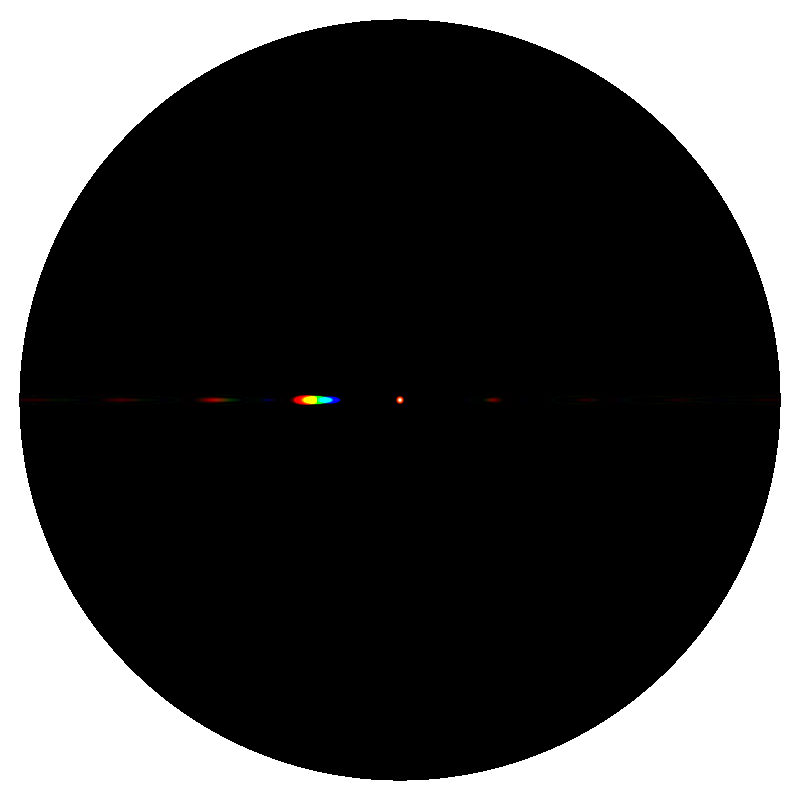
\includegraphics[scale=0.12]{results/PQapproach_vs_sampleAll/blaze/fftBlazeHeight_0.25Microns_allL_weak_scale_g=1.1.png}
    \label{fig:fullLambdaBlaze}
  }
~
  \subfigure[Full Lambda Sampling brightened: Blaze grating]{
    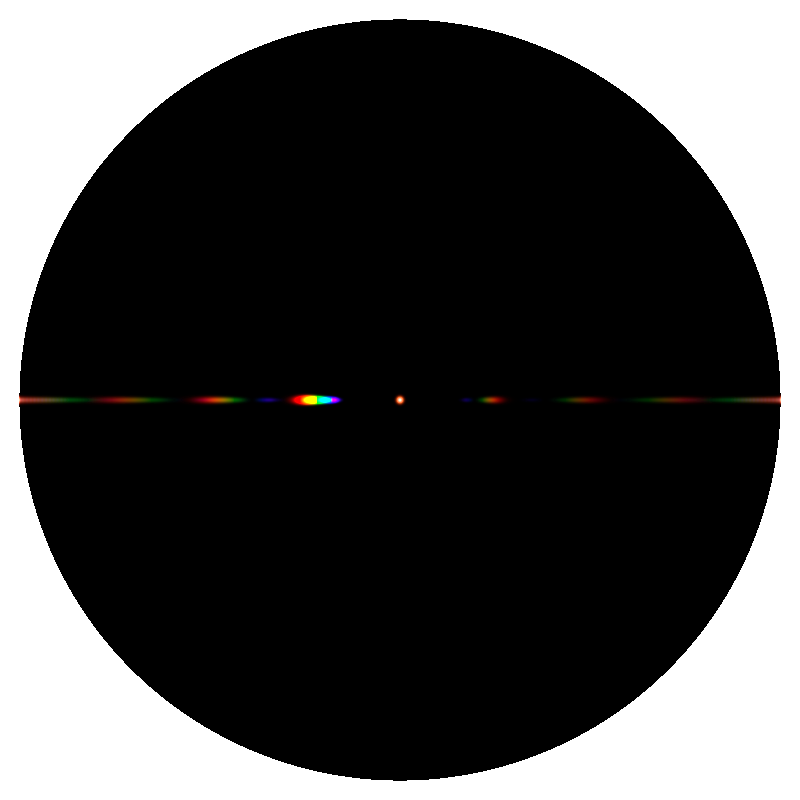
\includegraphics[scale=0.12]{results/PQapproach_vs_sampleAll/blaze/fftBlazeHeight_0.25Microns_allL_weak_scale_g=2.2_scale=100.png}
    \label{fig:fullLambdaBrightenedBlaze}
  }
~
  \subfigure[PQ Approach: Blaze grating]{
    \includegraphics[scale=0.12]{results/PQapproach_vs_sampleAll/blaze/pq.png}
    \label{fig:pqBlaze}
  }
  \label{pqBlaze}
  \caption{Blaze grating: PQ approach vs full lambda space sampling}
\end{figure}


%pq xeno
\begin{figure}[ht]
  \centering
  \subfigure[Full Lambda Sampling: Xeno grating $\theta_i = 0 degree$]{
    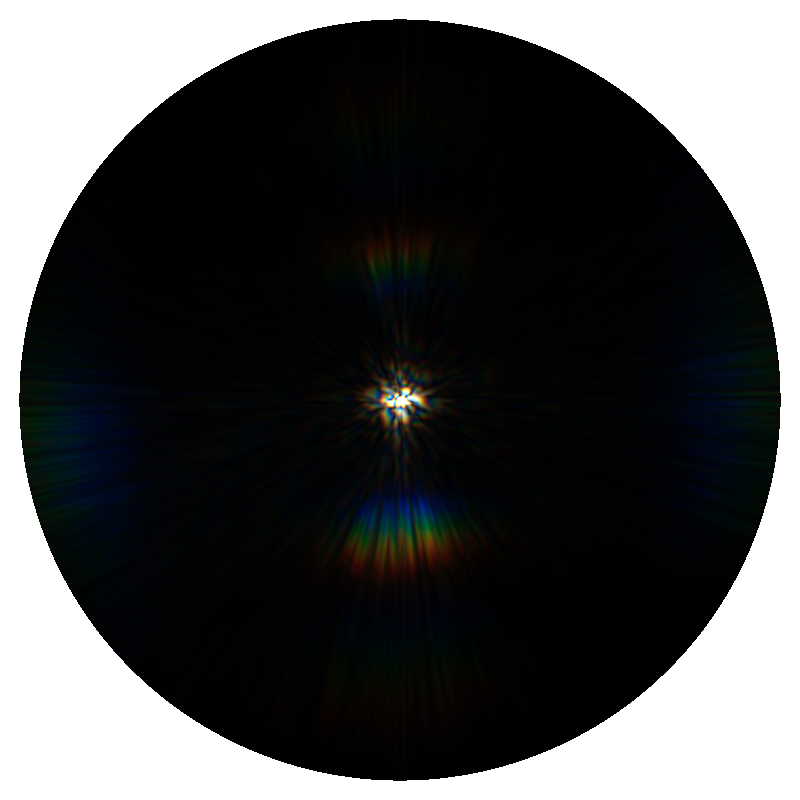
\includegraphics[scale=0.19]{results/PQapproach_vs_sampleAll/xeno/a_xeno_t_i=0.png}
    \label{fig:fullLambdaXenoti0}
  }
~
  \subfigure[PQ Approach: Xeno grating $\theta_i = 0 degree$]{
    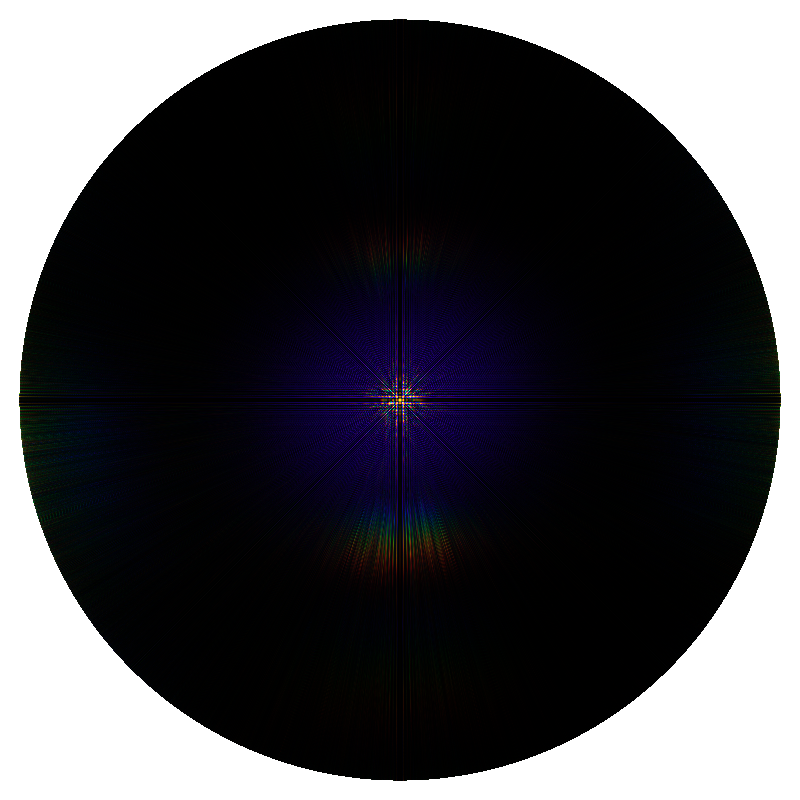
\includegraphics[scale=0.19]{results/PQapproach_vs_sampleAll/xeno/a_pq_t_i=0.png}
    \label{fig:pqXenoti0}
  }

  \subfigure[Full Lambda Sampling: Xeno grating $\theta_i = 10 degree$]{
    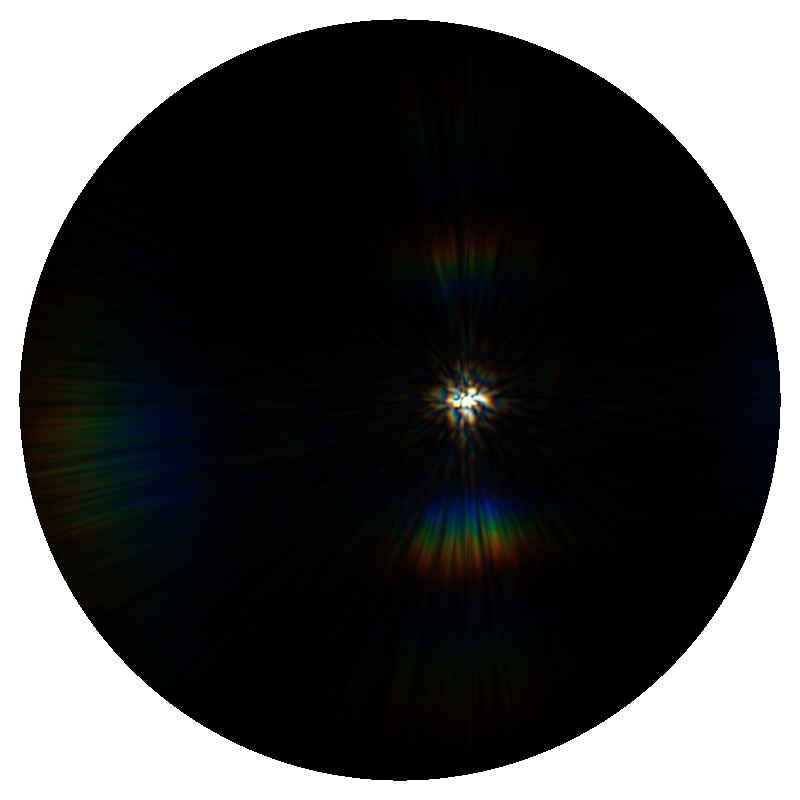
\includegraphics[scale=0.19]{results/PQapproach_vs_sampleAll/xeno/b_xeno_t_i=10.png}
    \label{fig:fullLambdaXenoti10}
  }
~
  \subfigure[PQ Approach: Xeno grating $\theta_i = 10 degree$]{
    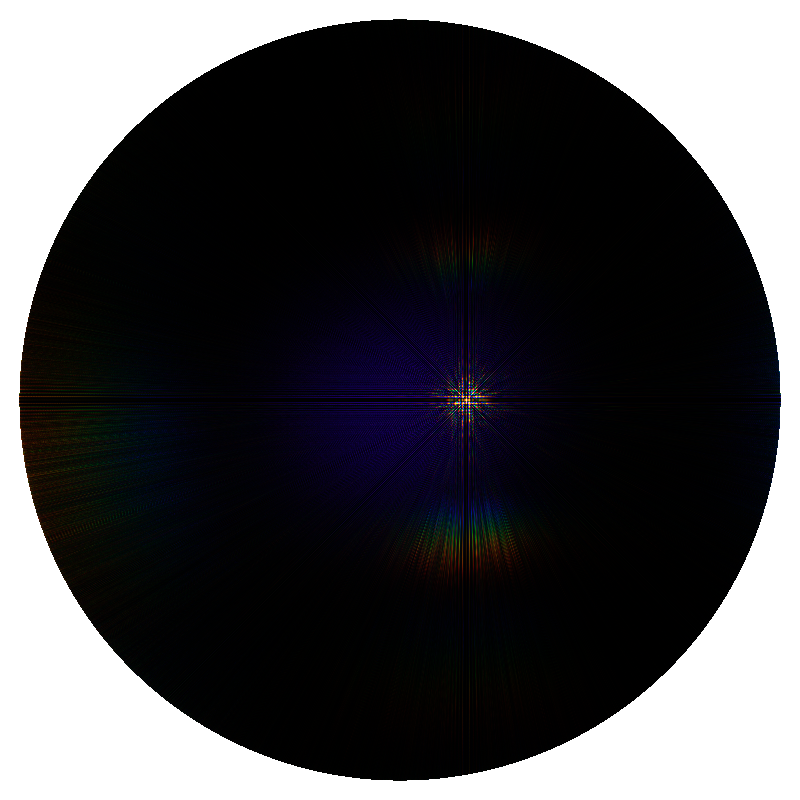
\includegraphics[scale=0.19]{results/PQapproach_vs_sampleAll/xeno/b_pq_t_i=10.png}
    \label{fig:pqXenoti10}
  }
  
  \subfigure[Full Lambda Sampling: Xeno grating $\theta_i = 20 degree$]{
    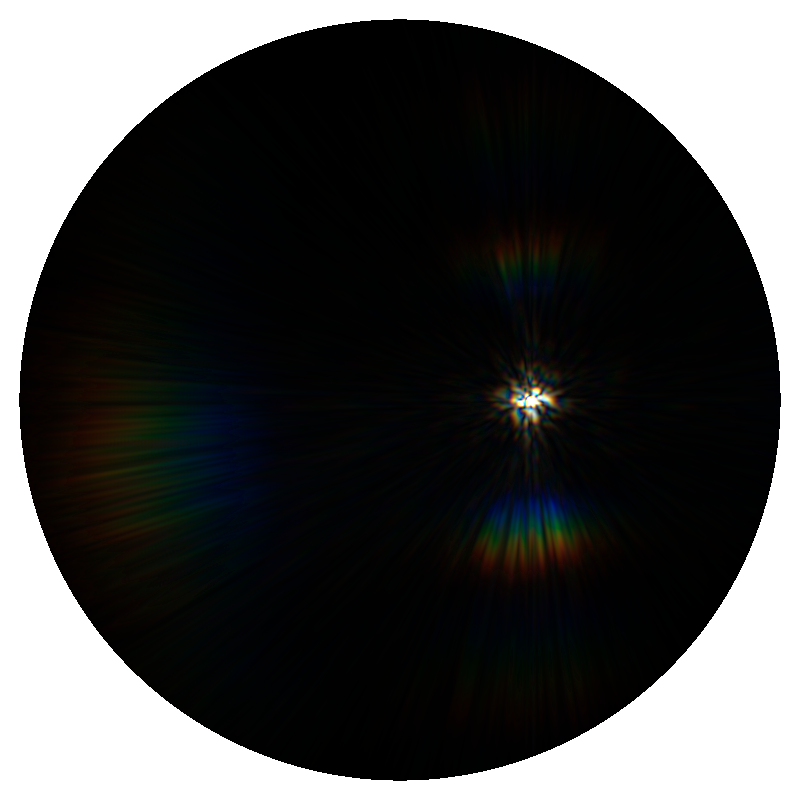
\includegraphics[scale=0.19]{results/PQapproach_vs_sampleAll/xeno/c_xeno_t_i=20.png}
    \label{fig:fullLambdaXenoti20}
  }
~
  \subfigure[PQ Approach: Xeno grating $\theta_i = 20 degree$]{
    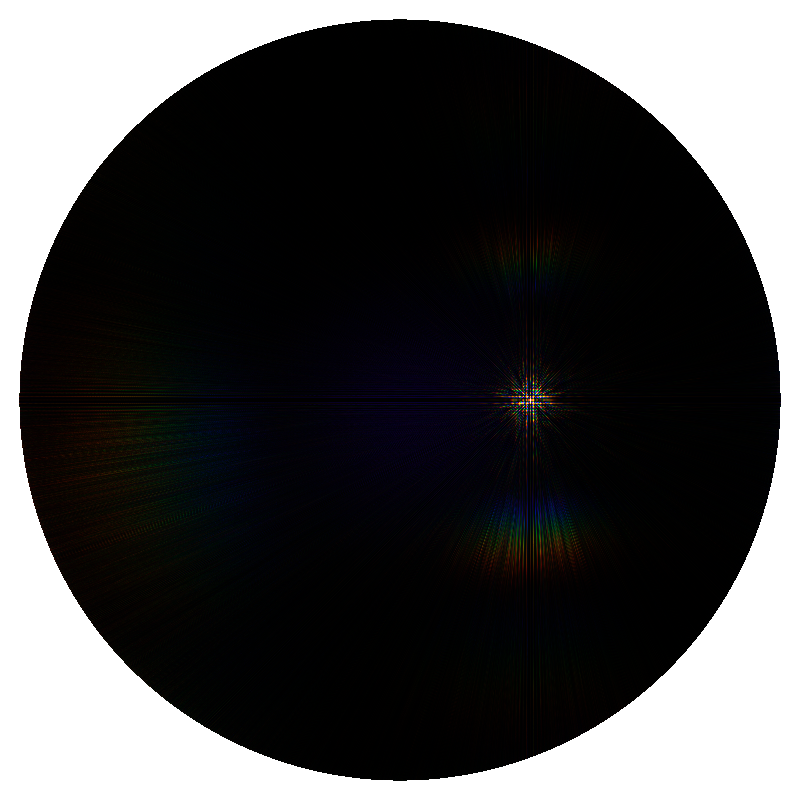
\includegraphics[scale=0.19]{results/PQapproach_vs_sampleAll/xeno/c_pq_t_i=20.png}
    \label{fig:pqXenoti20}
  }
  \label{pqXeno}
  \caption{Xeno grating: PQ approach vs full lambda space sampling}
\end{figure}

%pq elaphe
\begin{figure}[ht]
  \centering
  \subfigure[Full Lambda Sampling: Elaphe grating]{
    \includegraphics[scale=0.2]{results/PQapproach_vs_sampleAll/elaphe/elaph65.png}
    \label{fig:fullLambdaElaphe}
  }
~
  \subfigure[PQ Approach: Elaphe grating]{
    \includegraphics[scale=0.2]{results/PQapproach_vs_sampleAll/elaphe/pq.png}
    \label{fig:pqElaphe}
  }

  \label{pqElaphe}
  \caption{Elaphe grating: PQ approach vs full lambda space sampling}
\end{figure}

%sigma var
\begin{figure}[ht]
  \centering
  \subfigure[$\sigma_{s=3.25 \mu m}$]{
    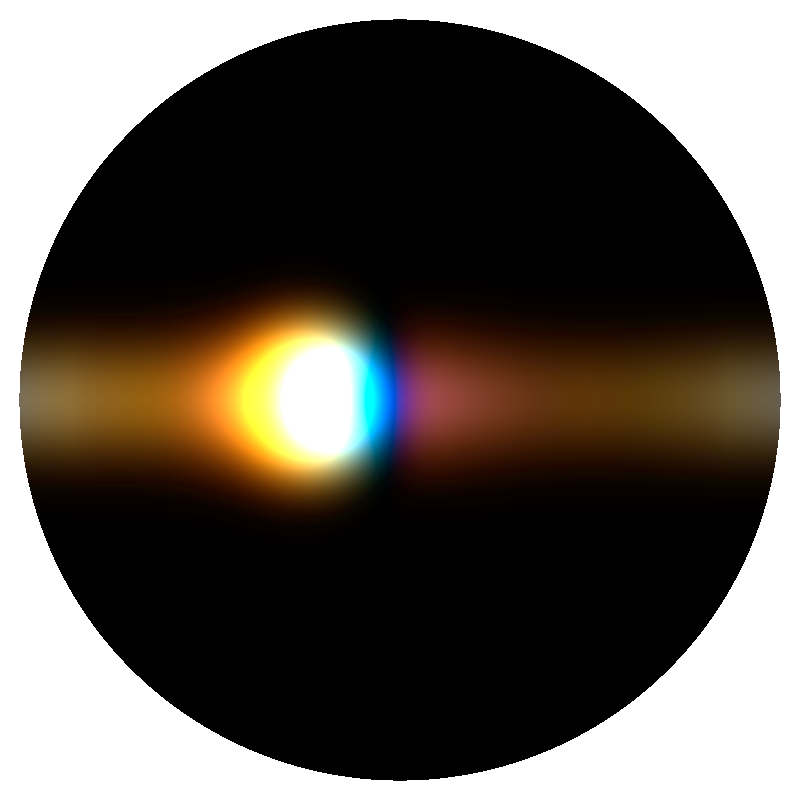
\includegraphics[scale=0.12]{results/sigma_sVariation/blaze/sigma_s=3.25.png}
    \label{fig:brdfmapsDiffSigmaStepsL1Blaze}
  }
~
  \subfigure[$\sigma_{s=6.5 \mu m}$]{
    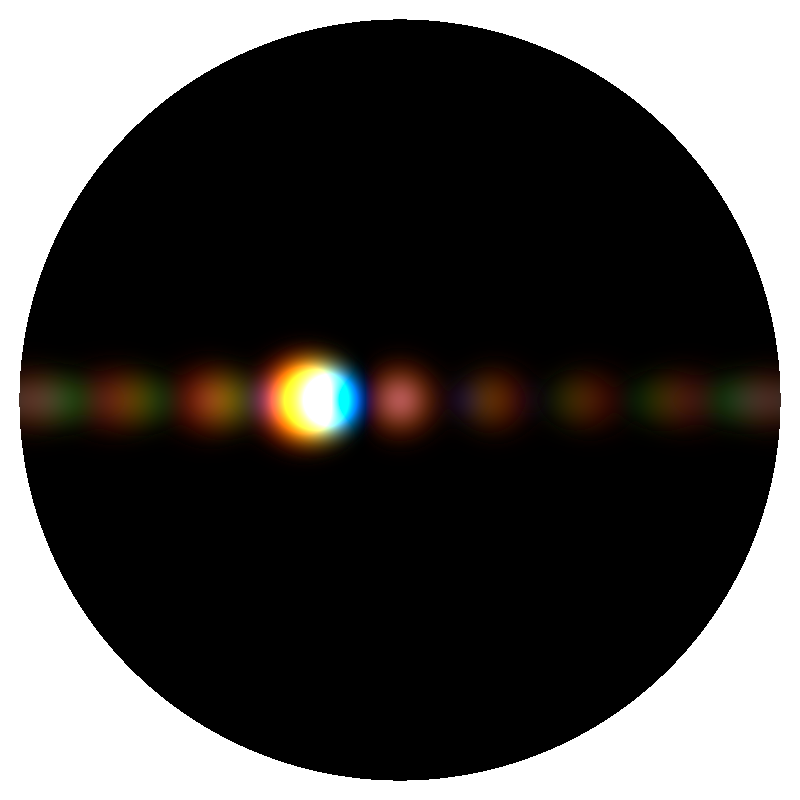
\includegraphics[scale=0.12]{results/sigma_sVariation/blaze/sigma_s=6.5.png}
    \label{fig:brdfmapsDiffSigmaStepsL5Blaze}
  }
~
  \subfigure[$\sigma_{s=15 \mu m}$]{
    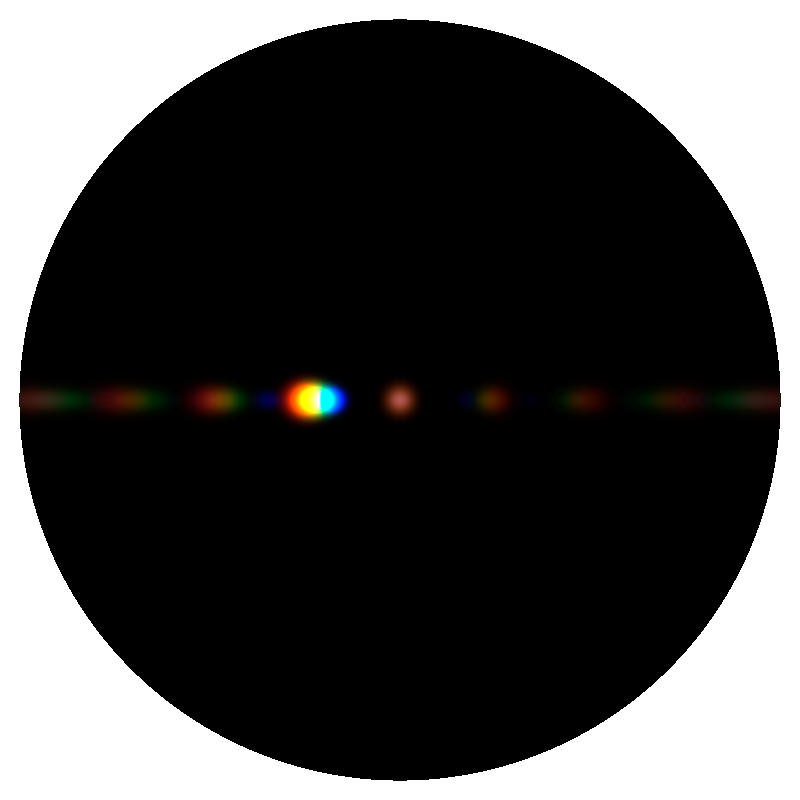
\includegraphics[scale=0.12]{results/sigma_sVariation/blaze/sigma_s=15.png}
    \label{fig:brdfmapsDiffSigmaStepsL10Blaze}
  }
  
  \subfigure[$\sigma_{s=30 \mu m}$]{
    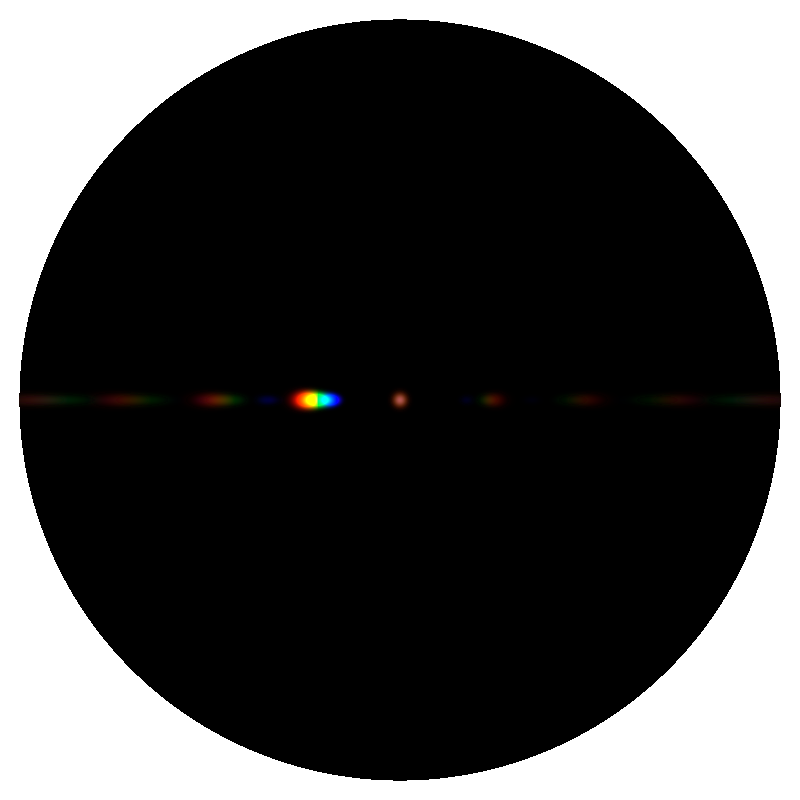
\includegraphics[scale=0.12]{results/sigma_sVariation/blaze/sigma_s=30.png}
    \label{fig:brdfmapsDiffSigmaStepsL25Blaze}
  }
~
  \subfigure[$\sigma_{s=45 \mu m}$]{
    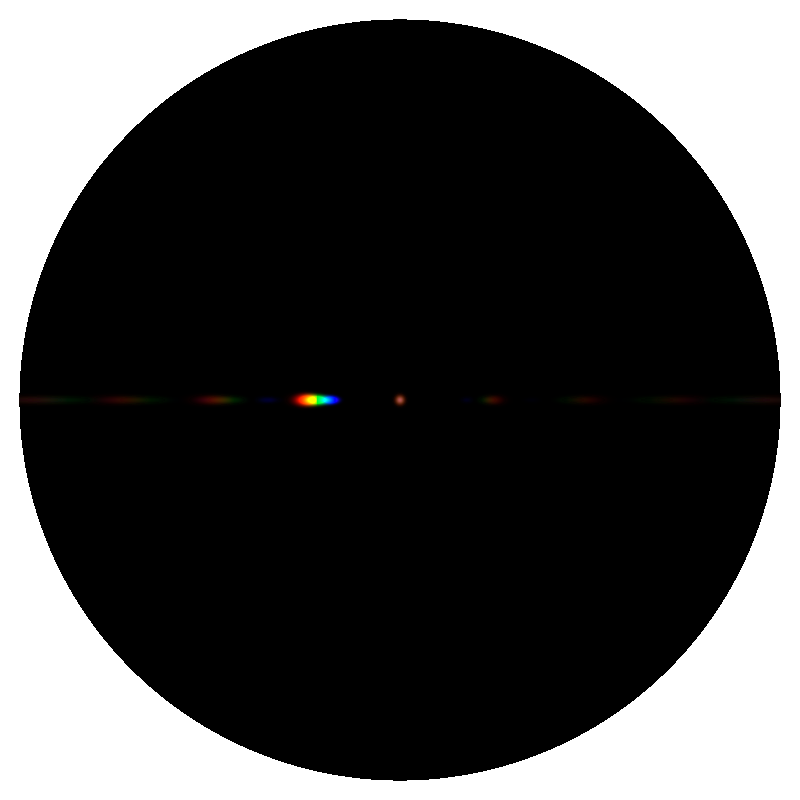
\includegraphics[scale=0.12]{results/sigma_sVariation/blaze/sigma_s=45.png}
    \label{fig:brdfmapsDiffSigmaStepsL50Blaze}
  }
~ 
  \subfigure[$\sigma_{s=65 \mu m}$]{
    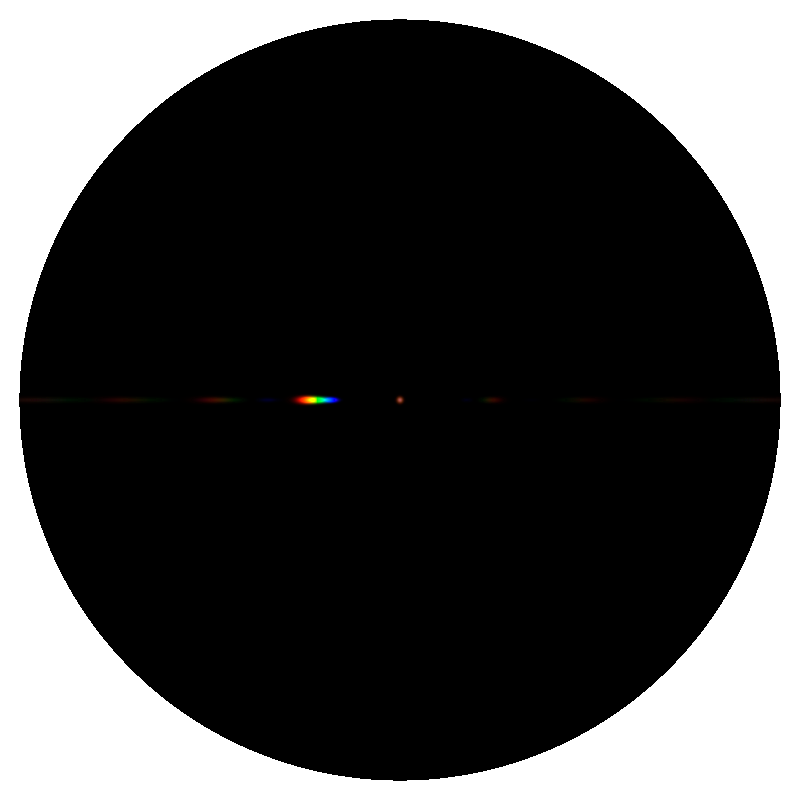
\includegraphics[scale=0.12]{results/sigma_sVariation/blaze/sigma_s=65.png}
    \label{fig:brdfmapsDiffSigmaStepsL100Blaze}
  }
  
  \label{brdfmapsDiffSigmaSizeBlaze}
  \caption{Blaze grating at $2.5 \mu m$: Different $\sigma_s$ sizes}
\end{figure}


%taylor var elaphe
\begin{figure}[ht]
  \centering
  \subfigure[$N=0$]{
    \includegraphics[scale=0.06]{results/taylorStepsVar/elaphe65/0.png}
    \label{fig:brdfmapsTaylorN0Elaphe65}
  }
~
  \subfigure[$N=1$]{
    \includegraphics[scale=0.06]{results/taylorStepsVar/elaphe65/1.png}
    \label{fig:brdfmapsTaylorN1Elaphe65}
  }
~
  \subfigure[$N=2$]{
    \includegraphics[scale=0.06]{results/taylorStepsVar/elaphe65/2.png}
    \label{fig:brdfmapsTaylorN2Elaphe65}
  }
~  
  \subfigure[$N=3$]{
    \includegraphics[scale=0.06]{results/taylorStepsVar/elaphe65/3.png}
    \label{fig:brdfmapsTaylorN3Elaphe65}
  }
~
  \subfigure[$N=4$]{
    \includegraphics[scale=0.06]{results/taylorStepsVar/elaphe65/4.png}
    \label{fig:brdfmapsTaylorN4Elaphe65}
  }

  \subfigure[$N=5$]{
    
\includegraphics[scale=0.06]{results/taylorStepsVar/elaphe65/5.png}
    \label{fig:brdfmapsTaylorN5Elaphe65}
  }
~  
  \subfigure[$N=6$]{
    \includegraphics[scale=0.06]{results/taylorStepsVar/elaphe65/6.png}
    \label{fig:brdfmapsTaylorN6Elaphe65}
  }
~  
  \subfigure[$N=7$]{
    \includegraphics[scale=0.06]{results/taylorStepsVar/elaphe65/7.png}
    \label{fig:brdfmapsTaylorN7Elaphe65}
  }
~  
  \subfigure[$N=8$]{
    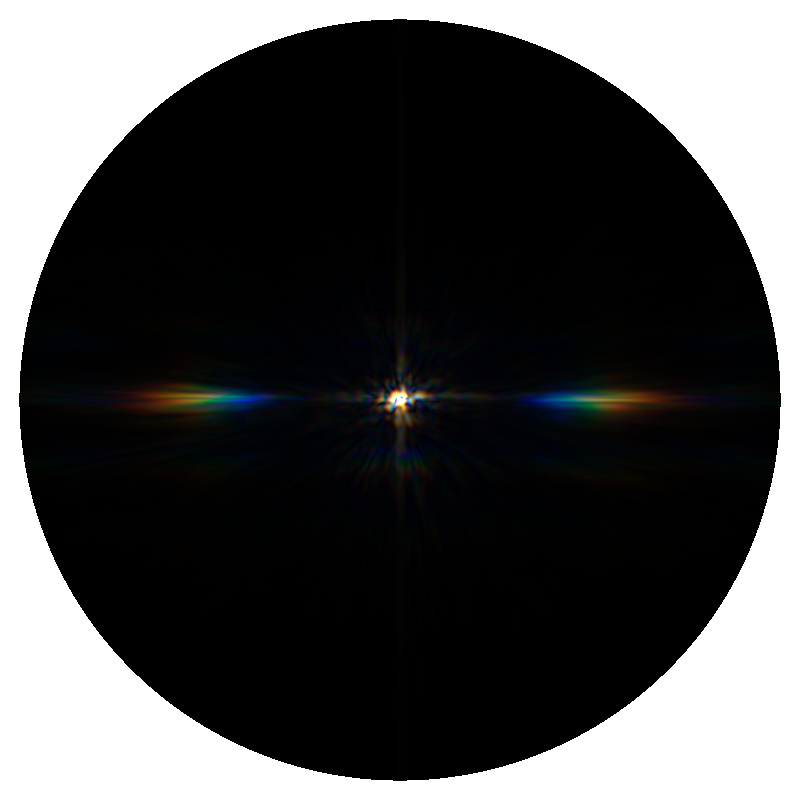
\includegraphics[scale=0.06]{results/taylorStepsVar/elaphe65/8.png}
    \label{fig:brdfmapsTaylorN8Elaphe65}
  }
~ 
  \subfigure[$N=9$]{
    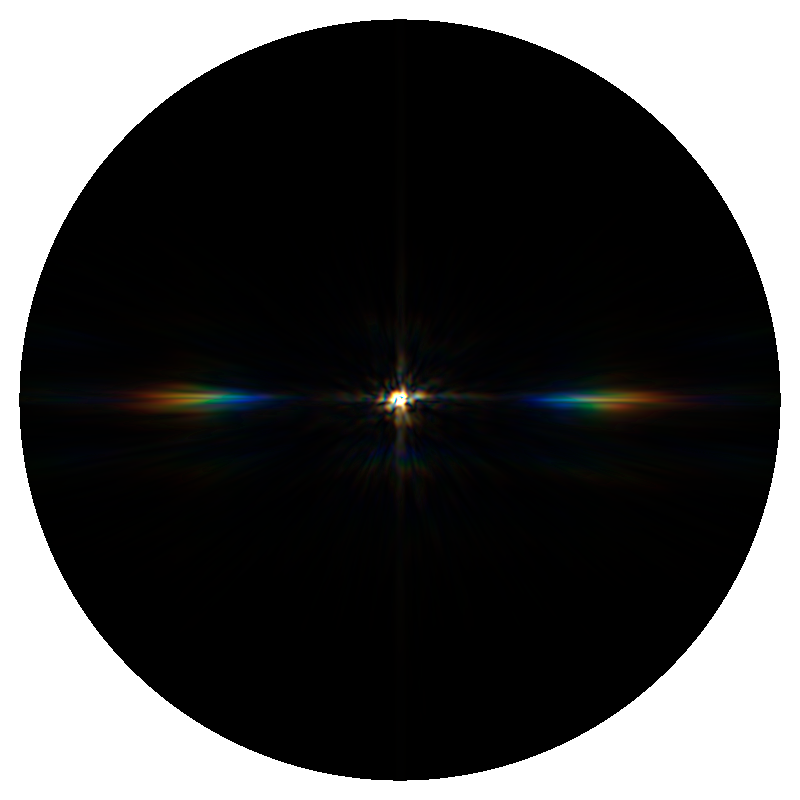
\includegraphics[scale=0.06]{results/taylorStepsVar/elaphe65/9.png}
    \label{fig:brdfmapsTaylorN9Elaphe65}
  }
  
  \label{brdfmapsTaylorIterationsElaphe65}
  \caption{Elaphe grating at $65 \mu m$: $N$ Taylor Iterations}
\end{figure}


%taylor var blaze
\begin{figure}[ht]
  \centering
  \subfigure[$N=0$]{
    \includegraphics[scale=0.06]{results/taylorStepsVar/blaze/0.png}
    \label{fig:brdfmapsTaylorN0Blaze}
  }
~
  \subfigure[$N=1$]{
    \includegraphics[scale=0.06]{results/taylorStepsVar/blaze/1.png}
    \label{fig:brdfmapsTaylorN1Blaze}
  }
~
  \subfigure[$N=2$]{
    \includegraphics[scale=0.06]{results/taylorStepsVar/blaze/2.png}
    \label{fig:brdfmapsTaylorN2Blaze}
  }
~  
  \subfigure[$N=3$]{
    \includegraphics[scale=0.06]{results/taylorStepsVar/blaze/3.png}
    \label{fig:brdfmapsTaylorN3Blaze}
  }
~
  \subfigure[$N=4$]{
    \includegraphics[scale=0.06]{results/taylorStepsVar/blaze/4.png}
    \label{fig:brdfmapsTaylorN4Blaze}
  }

  \subfigure[$N=5$]{
    
\includegraphics[scale=0.06]{results/taylorStepsVar/blaze/5.png}
    \label{fig:brdfmapsTaylorN5Blaze}
  }
~  
  \subfigure[$N=6$]{
    \includegraphics[scale=0.06]{results/taylorStepsVar/blaze/6.png}
    \label{fig:brdfmapsTaylorN6Blaze}
  }
~  
  \subfigure[$N=7$]{
    \includegraphics[scale=0.06]{results/taylorStepsVar/blaze/7.png}
    \label{fig:brdfmapsTaylorN7Blaze}
  }
~  
  \subfigure[$N=8$]{
    \includegraphics[scale=0.06]{results/taylorStepsVar/blaze/8.png}
    \label{fig:brdfmapsTaylorN8Blaze}
  }
~ 
  \subfigure[$N=9$]{
    \includegraphics[scale=0.06]{results/taylorStepsVar/blaze/9.png}
    \label{fig:brdfmapsTaylorN9Blaze}
  }
  
  \label{brdfmapsTaylorIterationsBlaze}
  \caption{Blaze grating at $2.5 \mu m$: $N$ Taylor Iterations}
\end{figure}

% brdf maps xeno angles
\begin{figure}[ht]
  \centering
  \subfigure[Xeno grating $\theta_i=0$]{
    \includegraphics[scale=0.12]{results/different_theta_i_angles/xenopeltis/xeno_t_i=0.png}
    \label{fig:brdfmapXenoti0}
  }
~
  \subfigure[Xeno grating $\theta_i=10$]{
    \includegraphics[scale=0.12]{results/different_theta_i_angles/xenopeltis/xeno_t_i=10.png}
    \label{fig:brdfmapXenoti10}
  }
~
  \subfigure[Xeno grating $\theta_i=20$]{
    \includegraphics[scale=0.12]{results/different_theta_i_angles/xenopeltis/xeno_t_i=20.png}
    \label{fig:brdfmapXenoti20}
  }
  \label{brdfmapsXenoDiffThetaIAngles}
  \caption{BRDF maps for Xeno grating: different $\theta_i$ angles}
\end{figure}


\section{Snake surface geometries}

\begin{figure}[ht]
  \centering
  \subfigure[Blaze grating]{
    \includegraphics[scale=0.12]{results/snakerenderings/compars/blaze.png}
    \label{fig:renderingBlazeGrating}
  }
~
  \subfigure[Elaphe grating]{
    \includegraphics[scale=0.12]{results/snakerenderings/compars/elaphe65.png}
    \label{fig:renderingElapheGrating}
  }
~
  \subfigure[Xeno grating]{
    \includegraphics[scale=0.12]{results/snakerenderings/compars/xeno65.png}
    \label{fig:renderingXenoGrating}
  }
  \label{renderingDifferentSnankeGratings}
  \caption{Diffraction of different snake skin gratings rendered on a snake geometry}
\end{figure}


\begin{figure}[ht]
  \centering
  \subfigure[$zoom = 0.1$]{
    \includegraphics[scale=0.2]{results/snakerenderings/zoomIn/elaphe65/0.1.png}
    \label{fig:renderingZoomElaphe01}
  }
~
  \subfigure[$zoom = 0.2$]{
    \includegraphics[scale=0.2]{results/snakerenderings/zoomIn/elaphe65/0.2.png}
    \label{fig:renderingZoomElaphe02}
  }
  
  \subfigure[$zoom = 0.5$]{
    \includegraphics[scale=0.2]{results/snakerenderings/zoomIn/elaphe65/0.5.png}
    \label{fig:renderingZoomElaphe05}
  }
~
  \subfigure[$zoom = 1.0$]{
    \includegraphics[scale=0.2]{results/snakerenderings/zoomIn/elaphe65/1.png}
    \label{fig:renderingZoomElaphe1}
  }
  
  \subfigure[$zoom = 1.5$]{
    \includegraphics[scale=0.2]{results/snakerenderings/zoomIn/elaphe65/1.5.png}
    \label{fig:renderingZoomElaphe15}
  }
~
  \subfigure[$zoom = 2.0$]{
    \includegraphics[scale=0.2]{results/snakerenderings/zoomIn/elaphe65/2.png}
    \label{fig:renderingZoomElaphe2}
  }
  \label{renderingDifferentZoomLevelsElaphe}
  \caption{Diffraction on Elaphe snake skin grating: Different camera zoom levels}
\end{figure}


